\chapter{Grundlagen}
\label{sec:grundlagen}
Dieses Kapitel behandelt die für diese Arbeit nötigen Grundlagen. Zunächst wird ein Überblick über grundlegende Begriffe vorgestellt. Das Responsive Webdesign und einige Merkmale für eine responsive Webseite in Bezug auf die zu entwickelnde Webanwendung werden erläutert. Dann werden das Web 2.0 und der entstandene Ausdruck \textit{Rich Internet Application} beschrieben. Anschließend gibt es die Unterschiede zwischen Thin Client und Thick Client.

\section{Grundlegende Begriffe}
\label{sec:grundlegende begriffe}

\subsection{Workshop}
\label{sec:workshop}
Workshop\footnote{bedeutet so viel wie \glqq Arbeitskreis oder -gruppe\grqq{} .} ist eine Veranstaltung, bei der sich eine bestimmte Anzahl von Personen teilnimmt, um außerhalb der Routinearbeit Fragen, Probleme und Themen zu bearbeiten. Jeder Workshop wird von einem Moderator geleitet. Bei größeren Gruppen (mehr als 15 Teilnehmer) ist der Einsatz von weiteren Moderatoren zu empfehlen. Die Teilnehmer handeln es sich in der Regel um Spezialisten oder Betroffene, die Ihr Fachwissen zu der behandelten Aufgabe einfließen lassen. Das Ziel ist dabei: Lösungsvorschläge für Aufgaben- oder Problemstellung zu generieren und Maßnahmenplan für die Umsetzung zu entwickeln.\bigskip

Der Moderator ist der aktiver Dienstleister der Gruppe. Er ist für die Vorbereitung sowie Organisation verantwortlich und soll die Gruppe am Ende zum Ziel führen. Seine Aufgaben bestehen unter anderem, Fragestellung gezielt zu formulieren, den Ablaufplan zu erstellen, Denkprozesse anzuleiten, Zeitplan einzuhalten und Ergebnisse zu dokumentieren. Er muss außerdem die stille Teilnehmer aktivieren sowie die dominante bremsen und darauf achten, dass die Gruppe bei Diskussionsrunden das Ziel nicht aus den Augen verliert.\bigskip

Nach Ansicht des Autors \cite{Boh2016} können Workshops in folgenden Projektphasen eingesetzt werden:

\begin{itemize} 
\item Kick-Off-Veranstaltung
\item Projektplanung-Prozess
\item Problemlösung
\item Entscheidungsfindung
\item Informationsaustausch
\item Teamentwicklung
\item Scrum
\item Projektabschluss
\end{itemize}

Die Gestaltung von Workshops spielt bei der Qualität der Ergebnisse eine große Rolle. Bei einem unstrukturierten Workshop kann dazu führen, dass er keine Motivation bei den Teilnehmer erregt, um sich an dem Workshop einzubringen und Ergebnisse zu erarbeiten. Um dagegen vorzugehen, können der Moderator je nach Dauer des Workshops folgenden kreative Workshop-Methoden anwenden, um Workshops effektiv und interaktiv zu gestalten:

\begin{itemize} 
\item World Cafe
\item Open Space
\item Six Thinking Hats
\item Fishbowl
\item Lego Serious Play
\end{itemize}
\medskip
Die genauen Beschreibungen zu den oben genannten Workshop-Methoden können im Blogpost von \par \cite{Cho2018} verfolgt werden.\bigskip
 
Wenn es darum geht, neue Ideen für Problemlösung, neue Produkten, neue Geschäftsideen oder Innovationen zu erzeugen, werden Kreativitätstechniken eingesetzt. Denn durch Kreativität werden Ideen generiert. Viele moderne Kreativitätstechniken haben sich im Laufe der Jahre etabliert. Dem Moderator steht deshalb eine Vielzahl von Kreativitätstechniken zur Verfügung. Der Klassiker und eine der beliebtesten unter allen Kreativitätstechniken ist wie bereits im Unterkapitel \textbf{\ref{sec:motivation}} erwähnt, das klassische Brainstorming. Da die vorliegende Arbeit eine Webanwendung zur Durchführung von Workshops behandelt, die das klassische Brainstorming digitalisieren soll, werde ich deshalb nicht auf die anderen vorhandenen Kreativitätstechniken eingehen. 

\newpage
\subsection{Brainstorming}
\label{sec:brainstorming}
Wie bereits im Unterkapitel \textbf{\ref{sec:motivation}} benannt, werden beim Brainstorming anhand eines konkreten Thema bzw. Problems Ideen, Einfälle und Vorschläge gesammelt. Es kommt dabei nicht auf die Qualität der Ideen an, sondern zunächst, dass möglichst viele Ideen generiert werden. Beim Brainstorming zählt die Quantität vor Qualität. Die Teilnehmer in der Gruppe sollen ihre Gedanken öffentlich frei äußern. Durch diesen öffentlichen Austausch, können mehr Ergebnisse produziert werden.\bigskip

Die Gruppengröße bei einer Brainstorming-Sitzung sollte nicht zu groß und zu klein sein.  \glqq Je nach Fachliteratur ist von Gruppengröße von 5 bis maximal 20 Personen die Rede\grqq{}. \cite{Pas2012}\bigskip

Nach \cite{Rei2007} läuft eine Brainstorming-Sitzung in folgenden Phasen ab: 

\begin{itemize} 
\item Vorbereitung:\\
Der Moderator stellt in dieser Phase die zu behandelte Frage und die Regeln vor. Bei Notwendigkeit kann ein oder mehrere Protokollant/en bestimmt werden.

\item Ideen sammeln:\\
Die Teilnehmer dürfen Ideen und Vorschläge frei äußern. Der Moderator muss in dieser Phase vor allem die stillere Teilnehmer motivieren und ermuntern. Die Kritik ist in dieser Phase untersagt. Die Ergebnisse werden dabei protokolliert. In der Regel werden die Ideen auf eine Notizzettel geschrieben und an die Wand gepinnt.

\item Zusammenfassung und Auswertung:\\
Das Brainstorming ist nun beendet und der Moderator wird die Gruppe zunächst die dokumentierte Ergebnisse präsentieren. Anschließend werden die Ideen gemeinsam mit der Gruppe ausgewertet, sortiert und geordnet. In dieser Phase ist Kritik erlaubt und darf geäußert werden. Am Ende dieser Phase soll eine Liste mit den gut bewerteten Ideen und Vorschläge entstehen.

\item Nachbereitung:\\
Ein Brainstorming fördert nur die Kreativität. Die Vorschlägen müssen danach umgesetzt und realisiert werden. Sonst helfen die Ideen nicht, wenn nichts daraus gemacht wird.
\end{itemize}

Damit eine Brainstorming-Sitzung erfolgreich verlaufen ist, sollten dabei folgenden Regeln eingehalten werden:

\begin{itemize} 
\item Unabhängig wie verrückt jede einzelne Idee ist, keine Kritik in der Sammlungsphase.
\item Quantität vor Qualität, je mehr Ideen desto besser.
\item Entwicklung oder Verbesserung von fremden Ideen ist willkommen.
\item Lass die Fantasie freien Lauf. Ungewöhnliche Ideen sind erwünscht.
\end{itemize}

\newpage
\subsection{TCP/IP}
\label{sec:tcp/ip}
Das Transmission Control Protocol (TCP) und das Internet Protocol (IP) bilden Grundlage für die gesamte Netzwerkkommunikation und legen demnach die grundlegende Technologien für das Internet dar.\bigskip

TCP nutzt für die Übertragung der Datenpakete das Übertragungsprotokoll IP, welches zur Vermittlungsschicht im TCP/IP-Referenzmodell gehört. Die Aufgabe von IP-Protokoll ist, die Datenpakete an den richtigen Rechner im Netzwerk zu transportieren. Die Datenpakete sind nicht anderes als Datagramme. Ein IP-Datagramm enthält unter anderem die IP-Adresse des Absenders und des Empfängers sowie weitere spezifische Übertragungsparameter (\textbf {Abbildung \ref{fig:datagramms}}). Ob alle versendeten Datagramme erfolgreich beim Empfänger angekommen sind, kann das IP-Protokoll jedoch nicht sicherstellen. Solche Fehlerbehandlungen, wie z.B. ob Pakete beim Empfänger tatsächlich angekommen sind, stellt die Transportschicht, allem voran TCP, sicher. (vgl. \cite{Kar.o.J.}] 

\begin{figure}[H]
  \begin{center}
    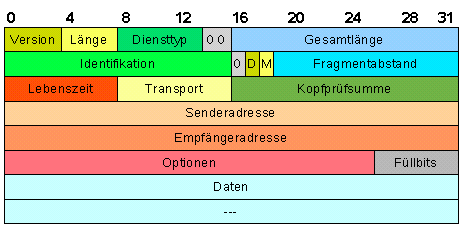
\includegraphics[width=9cm]{img/Datagramms.png}
	\caption{Aufbau eines Datagramms}
	\footnotesize\sffamily\textbf{Quelle:} \url{http://einstein.informatik.uni-oldenburg.de/rechnernetze/diagramm.htm} 
	\label{fig:datagramms}
  \end{center}   
\end{figure}

TCP ist eines der wichtigstens Protokolle der Transportschicht im TCP/IP-Referenzmodell und ist ein zuverlässiges, verbindungsorientiertes und paketvermittelndes Transportprotokoll, welches das Ziel hat, Datenverluste bei der Datenübertragung zu unterbinden, größere Datenmenge in kleinere Pakete zu zerlegen und die empfangene Datenpakete über Ports an den korrekten Anwendungen weiterzuleiten. Da sich TCP ein verbindungsorientiertes Protokoll handelt, definiert das TCP-Protokoll eine Ende-zu-Ende-Verbindung zwischen den Kommunikationspartnern im Netzwerk. (vgl. \cite{o.V.2019})\bigskip

Das TCP-Protokoll verwendet dabei das Verfahren namens \textit{Positive Acknowledgement (ACK) with ReTransmission\footnote{auf deutsch: positive Bestätigung mit erneuter Übertragung}}, um die Zuverlässigkeit der Datenübertragung sicherzustellen. Dies hat zu bedeuten, dass der Empfänger nach dem Erhalt der Daten dem Sender mit einer positiven Nachricht quittiert wird. Mit einer positiven Nachricht weiß der Sender, dass das Paket den Empfänger erreicht hat. Sollte von seitens der Empfänger keine positive Nachricht kommt, wird das Senden solange wiederholt, bis eine positive Antwort beim Sender eingegangen ist (\textbf {Abbildung \ref{fig:acknowledgement}}). (vgl. \cite{Hol2001})

\begin{figure}[H]
  \begin{center}
    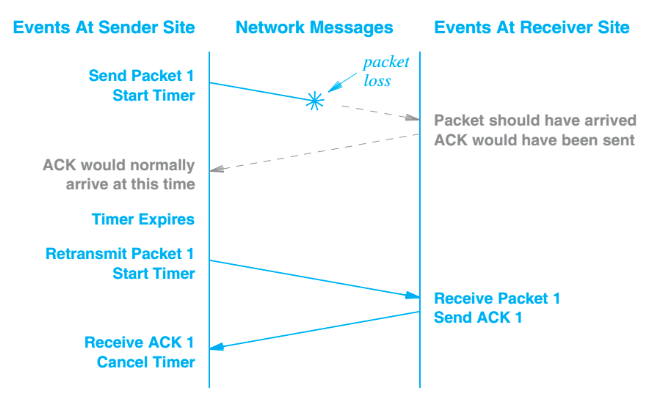
\includegraphics[width=9cm]{img/Acknowledgement.png}
	\caption{Zeitüberschreitung und erneute Übertragung bei Verlust eines Pakets}
	\footnotesize\sffamily\textbf{Quelle:} \url{http://lemoncisco.blogspot.com/2014/06/internetworking-with-tcpip-notes_25.html} 
	\label{fig:acknowledgement}
  \end{center}   
\end{figure}

Die folgende Abbildung (\textbf {Abbildung \ref{fig:tcp}}) zeigt die wichtigsten Protokolle im TCP/IP-Referenzmodell. Über der TCP- und IP-Schicht im TCP/IP-Referenzmodell befindet sich die Anwendungsschicht. Diese Schicht beinhaltet alle Protokolle auf Anwendungsebene, die auf TCP oder UDP aufsetzen. Die Anwendungsschicht stellt den Anwendungsprogrammen Dienste zur Verfügung. Das bekannteste Protokoll auf der Anwendungsschicht ist wohl das Hypertext Transfer Protocol (HTTP), welches den Zugriff auf die Webseiten ermöglicht.

\begin{figure}[H]
  \begin{center}
    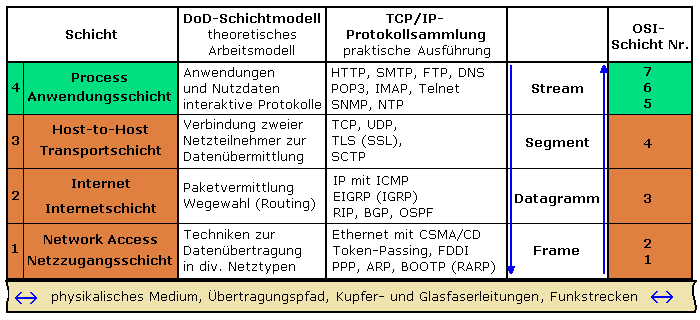
\includegraphics[scale=0.5]{img/tcp.png}
	\caption{Die wichtigsten Protokolle im TCP/IP-Referenzmodell}
	\footnotesize\sffamily\textbf{Quelle:} \url{https://www.elektroniktutor.de/internet/tcpip.html} 
	\label{fig:tcp}
  \end{center}   
\end{figure}

\newpage
\subsection{HTTP}
\label{sec:http}
Das Hypertext Transfer Protocol (HTTP) ist ein zustandsloses und unidirektionales Datenübertragungsprotokoll in einem Netzwerk. Es wird hauptsächlich eingesetzt, um die Dateien vom Server anzufordern und sie in den Browser zu laden und darzustellen. Bei HTTP handelt es sich um eine unverschlüsselte Kommunikation. Dies hat zur Folge, dass alle Informationen im Klartext gesendet werden. Für die verschlüsselte Verbindung bietet sich das sichere HyperText-Übertragungsprotokoll HTTPS\footnote{Hypertext Transfer Protocol Secure} an. HTTP arbeitet nach dem Client-Server-Modell (\textbf {Abbildung \ref{fig:client-server-modell}}). 

\begin{figure}[H]
  \begin{center}
    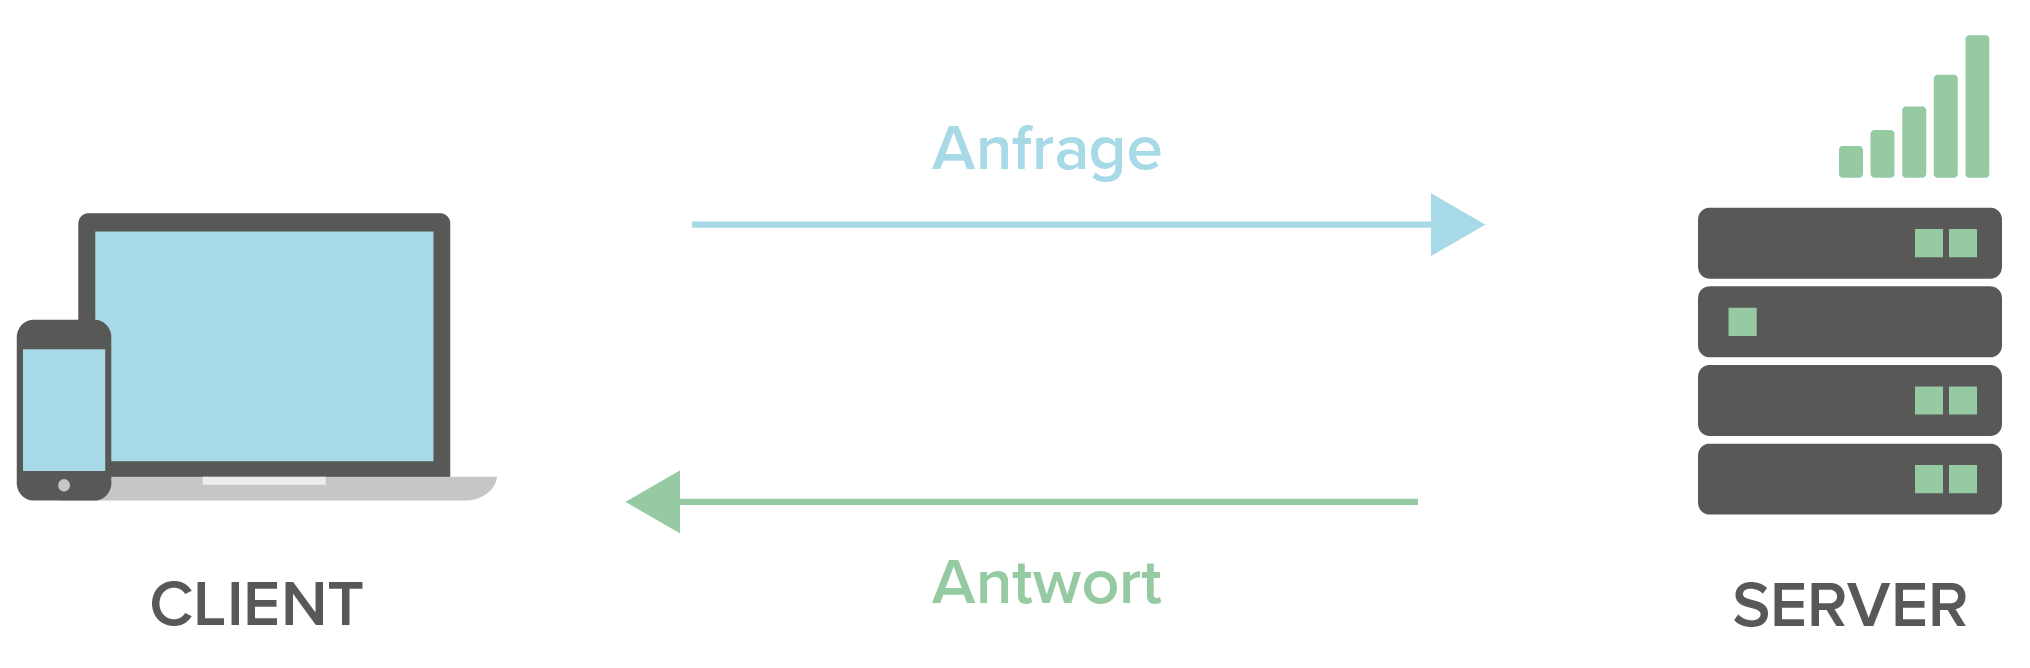
\includegraphics[scale=0.4]{img/client-server-modell.png}
	\caption{Das Client-Server-Modell}
	\footnotesize\sffamily\textbf{Quelle:} \url{https://www.placetel.de/ratgeber/client} 
	\label{fig:client-server-modell}
  \end{center}   
\end{figure}

Der Client (Webbrowser) sendet eine HTTP-Anfrage an den Port 80 des Servers (HTTP-Server). Dieser erledigt die Anfrage vom Client und schickt ihm eine Antwort zurück. Diese Kommunikation verläuft im Textformat. Die Anfrage- sowie die Antwortnachrichten bestehen aus einem Header und Daten. Der Header beinhaltet Steuerinformationen. Der Datenteil enthält den eigentlichen Inhalt der Seite. Nach Abarbeitung der Anfrage wird die Verbindung zwischen Client und Server abgeschlossen. Der Server steht also für die Bearbeitung von neuen Anfragen zur Verfügung. Um dem Server mitzuteilen, was er genau dem Client schicken soll, adressiert der Client bei der Anfrage eine Datei, die sich auf dem Server befindet muss. Dazu verwendet der Client eine URL\footnote{Uniform Resource Locator}. Ist diese Datei vom Client nicht vorhanden, antwortet der Server mit der Fehlermeldung (Error 404) zurück. Für eine zuverlässige Kommunikation verwendet HTTP das verbindungsorientierte Transportprotokoll TCP. (vgl. \cite{Lub2018})

\newpage
Eine URL ist wie folgt aufgebaut\footnote{vgl. \url{https://webdesigneinfuehrung.wordpress.com/tag-8/wie-ist-eine-url-aufgebaut/}}:

\begin{figure}[H]
  \begin{center}
    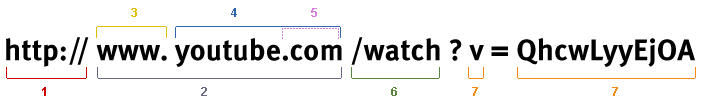
\includegraphics[scale=0.5]{img/url-aufbau.jpg}
	\caption{Aufbau einer URL}
	\footnotesize\sffamily\textbf{Quelle:} \url{https://webdesigneinfuehrung.files.wordpress.com/2013/10/url-aufbau.jpg} 
	\label{fig:url-aufbau}
  \end{center}   
\end{figure}

\begin{enumerate}
\item Das verwendete Protokoll (HTTP). Andere Protokolle könnten ebenfalls verwendet werden, wie HTTPS, FTP.
\item Es handelt sich um den Host oder Hostnamen.
\item Die Subdomain: www (World Wide Web).
\item Die Domain oder der Domainname. Dieser Name ist einmalig, wie eine Postanschrift.
\item beschreibt die Top-Level-Domain und bezieht sich auf das Ursprungsland der Webseite.
\item Der Pfad. Dieser verweist auf eine bestimmte Ressource (Datei, Verzeichnis) auf dem Server.
\item Parameter und Wert: v (Parameter), QhcwLyyEjOA (Wert).\\
Nach dem Pfad folgt in dem Beispiel ein URL-Parameter. Er wird durch ein Fragezeichen getrennt.
\end{enumerate}

\subsection{Ablauf einer HTTP-Verbindung}
\label{sec:ablauf einer http-verbindung}
Der Ablauf einer HTTP-Verbindung wird mit dem Beispiel eines Aufrufes einer Webseite im Webbrowser dargestellt. Das Aufrufen einer Webseite im Browser erfolgt hauptsächlich in vier Schritten:

\begin{figure}[H]
  \begin{center}
    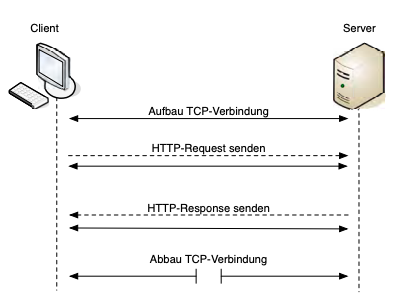
\includegraphics[scale=0.5]{img/http-request-response}
	\caption{Klassisches HTTP Request-Response-Paradigma nach \cite{Wöhr2004}}
	\label{fig:http-request-response}
  \end{center}   
\end{figure}

\newpage
\begin{enumerate}
\item Der Client baut eine TCP-Verbindung zum Server auf.
\item Der Client, in diesem Fall der Benutzer gibt z.B. eine Adresse (URL) in das Adressfeld seines Webbrowsers ein. Diese Adresse wird als HTTP-Request an der Server gesendet.
\item Der Server bearbeitet die Anfrage von dem Benutzer (Client) und antwortet ihm mit einer HTTP-Response zurück.
\item Nach dem Response baut der Server die Verbindung wieder ab.
\end{enumerate}

\subsection{AJAX}
\label{sec:ajax}
AJAX\footnote{Asynchronous JavaScript and XML} ermöglicht, dass sich die Daten zwischen Browser und Server im Hintergrund austauschen können, ohne die Seite komplett neu zu laden. Man spricht von einer asynchronen Datenübertragung zwischen Client und Server.\bigskip

Dabei ist das XMLHttpRequest\footnote{kurz: XHR}-Objekt in JavaScript für die Durchführung dieser asynchronen Datenübertragung zwischen Client und Server verantwortlich. XHR ist eine Schnittstelle zwischen JavaScript und Daten auf dem Server. Das XMLHttpRequest sendet eine HTTP-Anfrage an einen Webserver. Die Rückgabe vom Server kann ein JavaScript direkt per DOM\footnote{Document Object Modal} und CSS\footnote{Cascading Style Sheets} in das Dokument ergänzen oder verändert, ohne die Seite neu laden zu müssen. Die statischen Inhalte bleiben erhalten, während nur veränderliche Information ergänzt werden. Das spart vor allem Zeit, reduziert den Trafficverbrauch und ermöglicht dem Nutzer interaktiv mit dem Server zu kommunizieren.\bigskip

Nach \cite{o.V.2017} unterstützt XHR neben XML-Dokumente auch alle Textformate und kann eine Anfrage ebenfalls über HTTPS übermitteln.
Ein typisches Beispiel für die AJAX-Anwendung ist die Autovervollständigung von Google. Sobald der Nutzer die Daten im Suchfeld auf der Google Webseite eingibt, wird dabei automatisch die passende Vorschläge geliefert. 

\begin{figure}[H]
  \begin{center}
    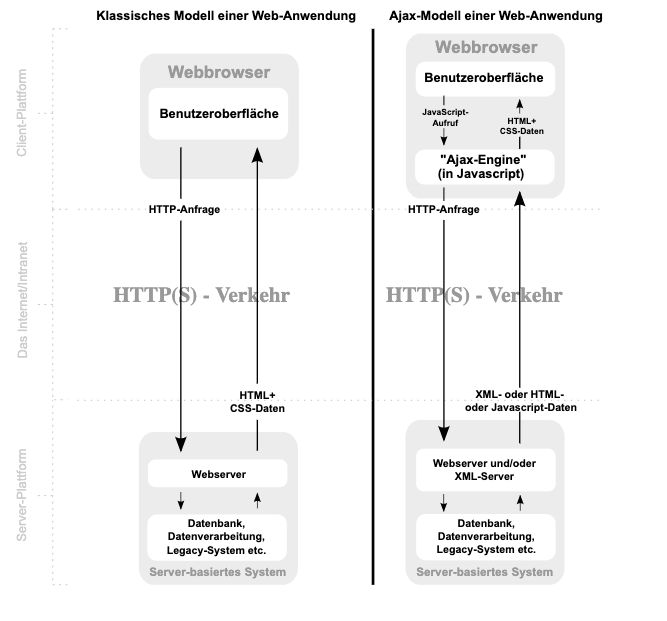
\includegraphics[scale=0.4]{img/ajax-modell}
	\caption{synchrone und asynchrone Kommunikation}
	\footnotesize\sffamily\textbf{Quelle:} By I, DanielSHaischt, CC BY-SA 3.0, \url{https://commons.wikimedia.org/w/index.php?curid=2223689} 
	\label{fig:ajax-modell}
  \end{center}   
\end{figure}

\subsection{Echtzeit}
\label{sec:echtzeit}
Der Begriff \glqq Echtzeit\grqq{} rückt immer mehr insbesondere bei bestimmten Webanwendungen in den Vordergrund auf. Was genau steckt hinter diesem Begriff? Lutz Schmitt hat in seiner Diplomarbeit diesen Begriff folgendermaßen definiert: \glqq Echtzeit beschreibt die Ausführung eines Prozesses in einem so kurzen Intervall, dass für die menschliche Wahrnehmung keine Zeit vergangen ist. Echtzeit beschreibt also das Phänomen der Reduzierung eines (Maschinen-)Prozesses auf einen Zeitpunkt.\grqq{} Ein Grund dafür, dass der Begriff Echtzeit in den letzten Jahren so viel an Bedeutung gewonnen hat, liegt darin, \glqq [...] dass viele Informationsverarbeitungsprozesse, die bis vor wenigen Jahren noch eine wahrnehmbare Dauer in Anspruch nahmen, so stark beschleunigt worden sind, dass sie eben nicht mehr wahrzunehmen sind. [...] Aus der Rechenzeit, die ein Computer für eine bestimmte Aufgabe benötigt, wird die Prozessverarbeitung in Echtzeit, die sofortige Erledigung ohne Verzögerung. [...] Anstatt auf die Maschine warten zu müssen, kann der Mensch unmittelbar weiterarbeiten.\grqq{} \cite{Lutz2006}\bigskip

In der heutigen Zeit, in der das Internet nicht mehr aus unserem Alltag wegzudenken ist, wurde der Begriff Echtzeit in den letzten Jahren so populär, vor allem bei Webanwendungen, die auf eine schnelle und latenzfreie Datenübertragung abhängig sind, wie z.B. Online-Spiele, Chat-Anwendungen oder kollaborative Webseite.

\newpage
Ein latenzfreier Informationsaustausch zwischen zwei Teilnehmern in einem Netzwerk ist mit dem bekannten Übertragungsprotokoll HTTP nicht gewährleistet. Dieses Protokoll arbeitet, wie bereits bekannt, nach dem Client-Server-Modell (\textbf{Abbildung \ref{fig:client-server-modell}}). Das hat zu bedeuten, dass nur der Client die Verbindung zum Server aufbaut, nie umgekehrt. Erst dann wenn die Verbindung zum Server erfolgreich hergestellt ist, folgt das Abschicken von Request- und Response-Nachrichten zwischen Client und Server. Man spricht hier von synchroner Übertragung. Nach dem Absenden der Antwortnachricht baut der Server die Verbindung anschließend wieder ab.\bigskip

Das Übertragungsprotokoll HTTP war in der Vergangenheit die perfekte Lösung für viele klassische Webanwendungen, um Kommunikation oder auch Interaktion zwischen zwei Kommunikationspartnern im Internet zu realisieren. Im Sinne der Echtzeit-Webanwendungen erfüllt dieses Übertragungsprotokoll jedoch nicht alle Anforderungen. Da es sich bei HTTP um eine synchrone Datenübertragung handelt, wird dabei die Benutzeraktivität unterbrochen, bis der Client die Antwort vom Server erhalten hat. Dieser Mangel kann durch AJAX mit der sogenannten asynchronen Datenübertragung behoben werden. Die Daten werden bei diesem Kommunikationsmodell im Hintergrund ausgetauscht, ohne dass die komplette Seite neu geladen werden muss. Trotz der Anwendung von AJAX bleibt das Hauptproblem weiterhin bestehen. Der Server kann bei HTTP nur auf Anfragen eines Clients reagieren, d.h. er wartet passiv auf Anforderungen. Eine Echtzeit-Anwendung soll durch die Interaktion vom Benutzer nicht unterbrochen werden. Häufig werden Echtzeit-Anwendungen durch Hacks (Polling oder Long Polling) simuliert. (vgl. \cite{Mar.o.D.})\bigskip

Beim Polling wird der Server in regelmäßigen Abständen (z.B. alle zwei Sekunden) vom Client angefragt, ob er neue Daten hat. Falls neue Daten vorliegen, wird der Server diese ohne Verzögerung an dem Client senden. Im Fall, dass keine Daten für die Anfrage vorliegen, wird dem Client vom Server mit einer leeren Nachricht geantwortet (\textbf{Abbildung \ref{fig:polling}}). (vgl. \cite{Mar2013})

\begin{figure}[H]
  \begin{center}
    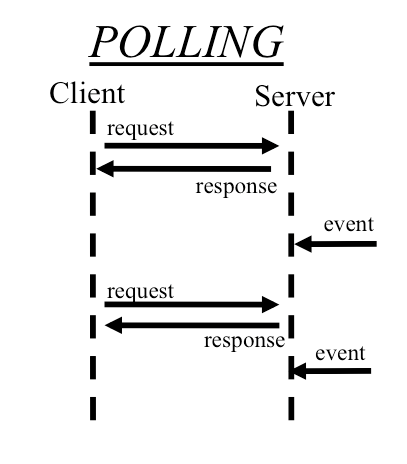
\includegraphics[scale=0.4]{img/polling}
	\caption{Polling}
	\footnotesize\sffamily\textbf{Quelle:} \url{https://www.heise.de/developer/imgs/06/6/7/6/2/3/3/Polling-61cb54a128001c08.png} 
	\label{fig:polling}
  \end{center}   
\end{figure}

Beim Long Polling wird der Server ebenfalls angefragt. Anders als beim Polling wird der Server diesmal bei nicht vorhandenen Daten solange warten, bis er sie an dem Client liefern kann. Das heißt, der Server hält die Verbindung solange offen, bis neue Daten für den Client verfügbar sind. Nachdem der Client die Daten erhalten hat, sendet er wieder eine Anfrage an den Server, um auf weitere Daten zu warten (\textbf{Abbildung \ref{fig:longPolling}}). (vgl. \cite{Mar2013})

\begin{figure}[H]
  \begin{center}
    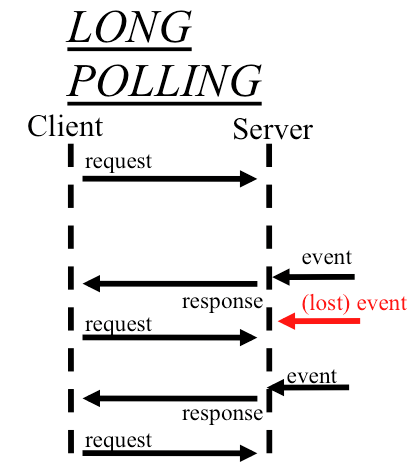
\includegraphics[scale=0.4]{img/longPolling}
	\caption{LongPolling}
	\footnotesize\sffamily\textbf{Quelle:} \url{https://www.heise.de/developer/imgs/06/6/7/6/2/3/3/LongPolling-616183343d043825.png} 
	\label{fig:longPolling}
  \end{center}   
\end{figure}

\newpage
Damit der Client und Server mit möglichst geringen Latenzen kommunizieren können, wird dafür eine bidirektionale Kommunikation benötigt. Mit dieser Art der Kommunikation können Daten in beide Richtungen gleichzeitig übertragen werden. Man bezeichnet diese Kommunikationsart als Vollduplex. Im Gegensatz zu Vollduplex erlaubt das Halbduplex-Verfahren keine gleichzeitige Kommunikation in beide Richtungen (vgl. \cite{Wiki2018}).\bigskip

\par
\begingroup
\leftskip=4em % Parameter anpassen
\rightskip\leftskip
\noindent \glqq HTTP ist von Natur aus ‘nur’ halbduplex. Das bedeutet, dass für die bidirektionale Kommunikation zwischen Browser und Server ein separater HTTP Request für jede Richtung benötigt wird. Das erzeugt natürlich einen Menge Overhead. [...] HTTP Request/Response Header können schnell ein paar Hundert Bytes veranschlagen. Hinzu kommt ab und an die eigentlich wertlose Information, dass es keine Änderungen am Zustand des Servers gab.\grqq{} \cite{Matt2011}
\par
\endgroup
\bigskip
Um dieses Problem zu lösen, wurde deshalb der Kommunikationsstandard namens WebSocket entwickelt.

\subsection{WebSocket}
\label{sec:websocket}
WebSocket wurde 2008 entwickelt. \glqq Chrome war 2009 der erste Browser, der WebSocket unterstützte; nach und nach folgten alle großen Wettbewerber. Seit 2011 ist WebSocket ein W3C\footnote{World Wide Web Consortium}-Standard.\grqq{} \cite{webSocket} \bigskip

WebSocket ist ein bidirektionaler und vollduplexer Kommunikationsstandard, der entwickelt wurde, \glqq[...] um eine bidirektionale Verbindung zwischen einer Webanwendung und einem WebSocket-Server bzw. einem Webserver, der auch WebSockets unterstützt, herzustellen.\grqq{} \cite{Wiki2019}\bigskip

Mit WebSocket werden Daten in beide Richtungen über einen Kommunikationskanal übertragen. Client und Server können gleichzeitig miteinander \glqq reden\grqq{}, sobald eine WebSocket-Verbindung besteht. WebSocket verwendet den gleichen Port wie HTTP, nämlich den Port 80. Es wird dabei ein WebSocket-Protokoll namens \textbf {Handshake} benutzt, um die Verbindung zwischen Client und Server aufzubauen. (vgl. \cite{Matt2011})

\newpage
Das Handshake-Verfahren funktioniert wie folgt:\bigskip

\textbf{Client:}

\begin{figure}[H]
  \begin{center}
    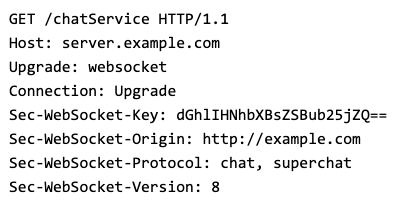
\includegraphics[scale=0.6]{img/clientWebsocket}
	\caption{Beispiel einer Client-Handshake-Anfrage}
	\footnotesize\sffamily\textbf{Quelle:} \url{https://www.heise.de/developer/artikel/WebSocket-Annaeherung-an-Echtzeit-im-Web-1260189.html?seite=all} 
	\label{fig:clientWebsocket}
  \end{center}   
\end{figure}

Im Prinzip ist es ein Aufsatz, der praktisch auf dem HTTP-Protokoll läuft. Wie in der \textbf{Abbildung \ref{fig:clientWebsocket}} zu sehen ist, schickt der Client eine normale GET-Anfrage an den Server und sagt dementsprechend auf der Serverseite, was er genau haben will. Mit dem \textbf{Upgrade} sagt der Client, dass er auf das WebSocket-Protokoll wechseln möchte. Dafür wird für den Verbindungsaufbau einen \textbf{Sec-WebSocket-Key} zum Server übermittelt. Bei diesem Key handelt es sich um eine Base64-encodierte Zeichenkette, welche vom Server benutzt wird, um den Verbindungsaufbau zu akzeptieren. (vgl. \cite{Matt2011})\bigskip

\textbf{WebSocket-Server:}

\begin{figure}[H]
  \begin{center}
    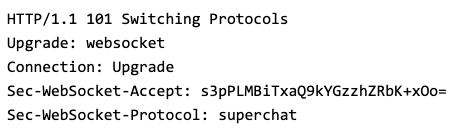
\includegraphics[scale=0.6]{img/serverWebsocket}
	\caption{WebSocket-Server Handshake}
	\footnotesize\sffamily\textbf{Quelle:} \url{https://www.heise.de/developer/artikel/WebSocket-Annaeherung-an-Echtzeit-im-Web-1260189.html?seite=all} 
	\label{fig:serverWebsocket}
  \end{center}   
\end{figure}

Der WebSocket-Server (\textbf{Abbildung \ref{fig:serverWebsocket}}) bearbeitet die Anfrage und antwortet mit dem HTTP-Status\- code 101 Switching Protocols. Dabei liefert er dem Client die Informationen mit, dass er das Upgrade akzeptiert hat (\textbf{Sec-WebSocket-Accept}). (vgl. \cite{Matt2011})

\newpage
\par
\begingroup
\leftskip=4em % Parameter anpassen
\rightskip\leftskip
\noindent \glqq Zusätzlich gibt der Server an, dass er das ‘superchat’-Protokoll kennt. Das hat den Vorteil, dass die Browseranwendung direkt gegen dieses Protokoll beziehungsweise diese API geschrieben wird, statt gegen die WebSocket-API. Entwickler, die mit der Programmierschnittstelle beziehungsweise dem anwendungsspezifischen Protokoll vertraut sind, brauchen keine neue API erlernen, um WebSocket-Anwendungen zu erstellen. Die clientseitige Schnittstelle des ‘superchat’-Protokolls kapselt die eigentliche Kommunikation mit dem WebSocket-Server.\grqq{} \cite{Matt2011}
\par
\endgroup

\begin{figure}[H]
  \begin{center}
    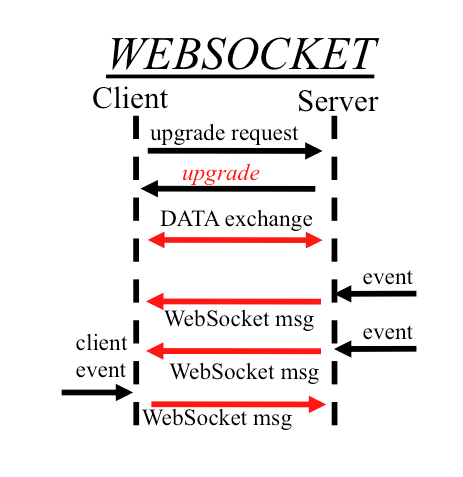
\includegraphics[scale=0.4]{img/webSocketHandshake}
	\caption{Das WebSocket-Handshake}
	\footnotesize\sffamily\textbf{Quelle:} \url{https://www.heise.de/developer/imgs/06/6/7/6/2/3/3/WebSocket-a70195c3f57b1308.png} 
	\label{fig:webSocketHandshake}
  \end{center}   
\end{figure}

Nach dem Handshake besteht eine persistente Verbindung zwischen Client und Server und beide können jederzeit mit dem Senden von Daten beginnen (\textbf{Abbildung \ref{fig:webSocketHandshake}}). Eine WebSocket-Verbindung erkennt man an das neue URL-Schema. Statt wie gewohnt das \glqq http:\grqq{} oder für sichere HTTP-Verbindungen das \glqq https:\grqq{} als Protokoll anzugeben, wird bei einer WebSocket-Verbindung das \glqq ws:\grqq{} verwenden. Für sichere Verbindungen steht das \glqq wss:\grqq{} zur Verfügung.\bigskip

Zusammenfassend lässt sich sagen, dass WebSocket ein geeigneter Protokoll ist, um \bigskip

\par
\begingroup
\leftskip=4em % Parameter anpassen
\rightskip\leftskip
\noindent \glqq [...] die komplexen Probleme des ‘Echtzeit-Web’, wie Latenz oder Netzverkehr, anzugehen. WebSocket wird jedoch nicht als ein ‘besseres AJAX’ entwickelt. Ebenfalls stellt WebSocket keinen 1:1-Ersatz für HTTP dar, sondern bietet vielmehr einen effizienten, bidirektionalen Kommunikationskanal an. Die Integration von ‘Echtzeit’ innerhalb von Webanwendungen ist nicht mehr an Hacks und Workarounds gebunden, sondern erfolgt auf Basis eines standardisierten, effizienten und bidirektionalen Protokolls. Wichtig ist hierbei, dass man sämtliche TCP/UDP-Protokolle auf Basis von WebSocket zum Browser bringen kann. Der Abstraktionsgrad zukünftiger Webanwendungen steht damit den Desktop-Anwendungen in nichts nach.\grqq{} \cite{Matt2011}
\par
\endgroup

\subsection{jQuery}
\label{sec:jQuery}
jQuery ist eine JavaScript-Bibliothek, die Klassen und Methoden zur Verfügung stellt, um die Arbeit mit JavaScript zu vereinfachen. jQuery ist nicht nur kompakter und komfortabler als JavaScript, sondern außerdem browserübergreifend, was bei JavaScript in der Vergangenheit nicht immer der Fall war. jQuery vereinfacht viele JavaScript-Funktionen, die bei der Webentwicklung oft verwendet wird. Wie JavaScript ermöglicht jQuery auch den Zugriff auf DOM-Elemente. DOM-Elemente können gezielt angesprochen und manipuliert werden. (vgl. \cite{Ste2019})\bigskip

Laut \cite{Wiki2019b} ist jQuery die meist verwendete JavaScript-Bibliothek und wird auf rund 70\% der 10000 meistbesuchten Webseiten eingesetzt.\bigskip

Das DOM versteht sich als die Schnittstelle für den Zugriff auf den Tags, Attribute und Inhalte von HTML- oder XML-Dokumenten und wird vom W3C definiert. Mithilfe von Selektoren und dem DOM können die HTML-Elemente aufgerufen, verändert, hinzugefügt und gelöscht werden. Die Elemente können über id- oder class-Attribute selektiert werden. 

\begin{figure}[H]
  \begin{center}
    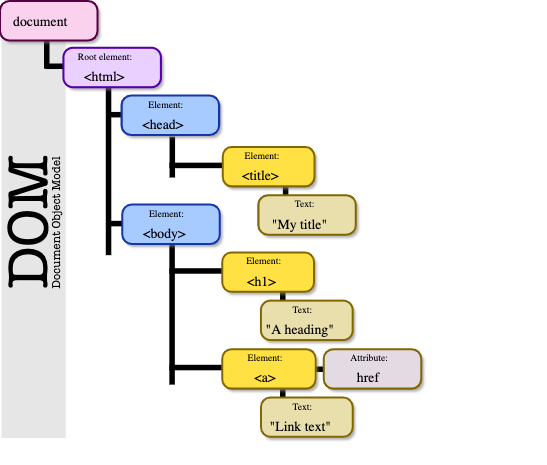
\includegraphics[scale=0.5]{img/dom}
	\caption{DOM - Elementenbaum einer Webseite}
	\footnotesize\sffamily\textbf{Quelle:} By Birger Eriksson - Own work, CC BY-SA 3.0, \url{https://commons.wikimedia.org/w/index.php?curid=18034500} 
	\label{fig:dom}
  \end{center}   
\end{figure}

\newpage
Weitere jQuery-Funktion:
\begin{itemize}
\item Event Handling
\item Form Handling
\item AJAX
\item JSON
\item Collect und Select
\item Animationen
\end{itemize}

\section{Responsive Webdesign}
\label{sec:responsive webdesign}
Um eine Webseite geräteübergreifend zu gestalten, benötigt sie ein \glqq Responsive Webdesign\grqq{}. Beim Responsive Webdesign handelt es sich um eine reaktions- und anpassungsfähige Weboberfläche, so dass diese ein einheitliches Anzeigen von Inhalten sowie den strukturellen Aufbau einer Webseite auf dem Desktop-Computer, Tablet und Smartphone bietet. Laut \cite{Wiki2019c} wurde der Begriff im Jahr 2010 vom amerikanischen Webdesigner Ethan Marcotte erfunden.\bigskip

Da es zu jener Zeit kaum internetfähige Mobilgeräte auf dem Markt gab, waren die meisten Webseiten statisch und nur für Desktop-Computer entwickeln worden. Um eine Webseite für Mobilgeräte anzubieten, musste separat eine mobile Webseite entwickelt werden.\bigskip

Erst mit der Einführung des IPhones von Apple im Januar 2007\footnote{vgl. \url{https://de.wikipedia.org/wiki/IPhone_(erste_Generation)}} war es für den Benutzer möglich, mobil ins Internet zu gehen. Erstmals verfügte ein Mobilgerät einen vollwertigen Webbrowser und war über einen Touchscreen verfügbar. Viele Firmen folgten dem Beispiel von Apple und wenige Jahre später brachten sie eine Menge an verschiedenen Mobilgeräten mit individuellen Displaygrößen auf dem Markt.\bigskip

Seit der Einführung der Smartphones, Tablets und mit der steigenden mobilen Internetnutzung ist ein Responsive Webdesign heutzutage nicht nur ein nettes Feature sondern ein Pflichtprogramm für jeden Webseitenbetreiber. Für neue Webseiten liegt es auf der Hand, wie man vorgehen sollte, für bestehende statische Webseiten ist der Aufwand sehr groß, diese auf eine responsive Webseite umzustellen, da eventuell die komplette Seite neu entwickeln werden muss.\bigskip

Die vorliegende Arbeit soll auf verschiedenen Geräten optimal angezeigt werden können. Als \glqq responsive\grqq{} Webseite muss sie unter anderem folgende Eigenschaften haben.

\begin{itemize}
\item \textbf{flexibles Grid\footnote{aus dem Englischen für das Gestaltungsraster bekannt}-Layout}\par
Seiten und Elemente, wie Bilder oder Textblöcke, müssen sich der Bildschirmauflösung des mobilen Endgeräts anpassen. Hier werden für die Elemente und Seiten prozentuale statt fester Pixelwerte verwendet.
\item \textbf{keine festen Schriftgrößen}\par
Fließtexte und Headlines müssen so angepasst werden, dass sie sowohl auf dem PC als auch auf Smartphones und Tablet gut lesbar sind. Hier ist eine feste Schriftgröße nicht geeignet. Es wird daher mit prozentualen Werten oder Maßen wie em gearbeitet.
\end{itemize}

\section{Web 2.0}
\label{sec:web2.0}
Das Web 2.0 wird als \glqq Mitmach-Netz\grqq{} verstanden. Es ist eine Revolution hinsichtlich der Nutzung des World Wide Web, bei der Internetnutzer nicht mehr wie früher, nur die Inhalte des Internets konsumieren, sondern auch eigene Inhalte selbst produzieren, wie Videos und Fotos einstellen oder Texte schreiben. Durch seine Beteiligung im Web ist der Internetnutzer selbst ein Teil des Internets.\bigskip 

Beim Web 2.0 handelt es sich dabei nicht um eine neue Technologie, sondern vielmehr um die Weiterentwicklung des Internets. Dazu zählt beispielsweise der vermehrte Einsatz der AJAX-Technologie, die eine asynchrone Datenübertragung zwischen Client und Server ermöglicht. Oder der Einsatz von Abonnementdienste (Web-Feeds), welche eine grundlegende Eigenschaft für die neue Generation des World Wide Webs sind. (vgl. \cite{o.V.2008})\bigskip

Der Begriff Web 2.0 ist durch seinen Artikel \glqq What is Web 2.0\grqq{} von amerikanischen Verleger Tim O’Reilly in 2005 bekannt geworden\footnote{vgl. \url{https://www.oreilly.com/pub/a/web2/archive/what-is-web-20.html}}.

\begin{figure}[H]
  \begin{center}
    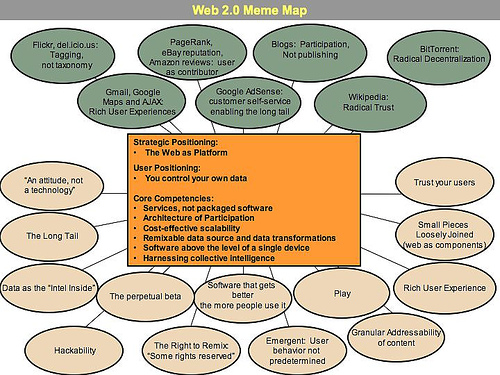
\includegraphics[scale=0.6]{img/web2_map.jpg}
	\caption{Das Konzept Web 2.0 nach einer Brainstorming-Sitzung}
	\footnotesize\sffamily\textbf{Quelle:} \url{http://www.siliconbeat.com/entries/meme-map.jpg} 
	\label{fig:web2_map}
  \end{center}   
\end{figure}

\textbf{Die Abbildung \ref{fig:web2_map}} zeigt ein Konzept von Web 2.0, die mit einem Brainstorming zwischen O’Reilly und MediaLive International entwickelt wurde. \textbf{Die Abbildung \ref{fig:Web1vsWeb2}} beschreibt einige Beispiele für die Bedeutung von Web 2.0, die im ersten Brainstorming zwischen O’Reilly und MediaLive International formuliert wurden.

\begin{figure}[H]
  \begin{center}
    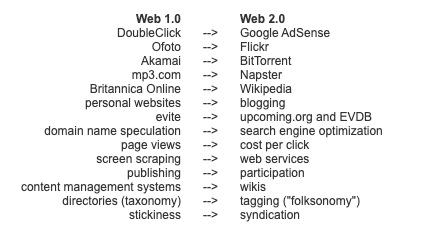
\includegraphics[scale=0.7]{img/web1_vs_web2}
	\caption{Die Bedeutung von Web 2.0}
	\footnotesize\sffamily\textbf{Quelle:} \url{https://www.oreilly.com/pub/a/web2/archive/what-is-web-20.html?page=1#mememap} 
	\label{fig:Web1vsWeb2}
  \end{center}   
\end{figure}

\newpage
Außerdem stellte O’Reilly sieben Merkmale vor, die kennzeichnend für Web 2.0 sind:

\begin{itemize}
\item \textbf{Das Web als Plattform:}
\begin{itemize}
\item Das Web als Plattform ähnlich wie ein Betriebssystem.
\end{itemize}
\item \textbf{Kollektive Intelligenz:}
\begin{itemize}
\item Verlinkung der Daten und Seiten untereinander.
\end{itemize}
\item \textbf{Daten als nächstes Intel Inside:}
\begin{itemize}
\item Die gesammelte Daten sind die Basis einer Webanwendung und sind wichtiger und wertvoller als eine einzelne Anwendung.
\end{itemize}
\item \textbf{Softwarelebenszyklus:}
\begin{itemize}
\item Software wird nicht mehr als Produkt ausgeliefert, sondern als Service.
\end{itemize}
\item \textbf{Lightweight Programming Models:}
\begin{itemize}
\item Daten werden durch Web-Services bereitgestellt.
\end{itemize}
\begin{itemize}
\item Die Daten werden über den Web-Services wie RSS oder REST-basierten Web-Services verteilt oder ausgetauscht.
\end{itemize}
\item \textbf{Software über Gerätegrenzen hinaus:}
\begin{itemize}
\item Geräteunabhängige Anwendungen, z.B. nicht nur für den PC sondern auch mobile Geräte.
\end{itemize}
\item \textbf{Rich User Experiences:}
\begin{itemize}
\item Benutzerführung mit interaktiver Benutzeroberfläche, die sich kaum von einem Desktop-Programm unterscheiden.
\end{itemize}
\begin{itemize}
\item AJAX-Technologie.
\end{itemize}
\end{itemize}

\newpage
\section{Rich Internet Applications}
\label{sec:rich internet applications}
